\documentclass{standalone}
\usepackage{tikz}
\usetikzlibrary{shapes,arrows,positioning,fit,backgrounds,shadows,decorations.pathmorphing,decorations.pathreplacing}
\usetikzlibrary{calc,intersections,through,backgrounds,matrix}
\usetikzlibrary{arrows.meta, calc, positioning, shapes.geometric}

\begin{document}
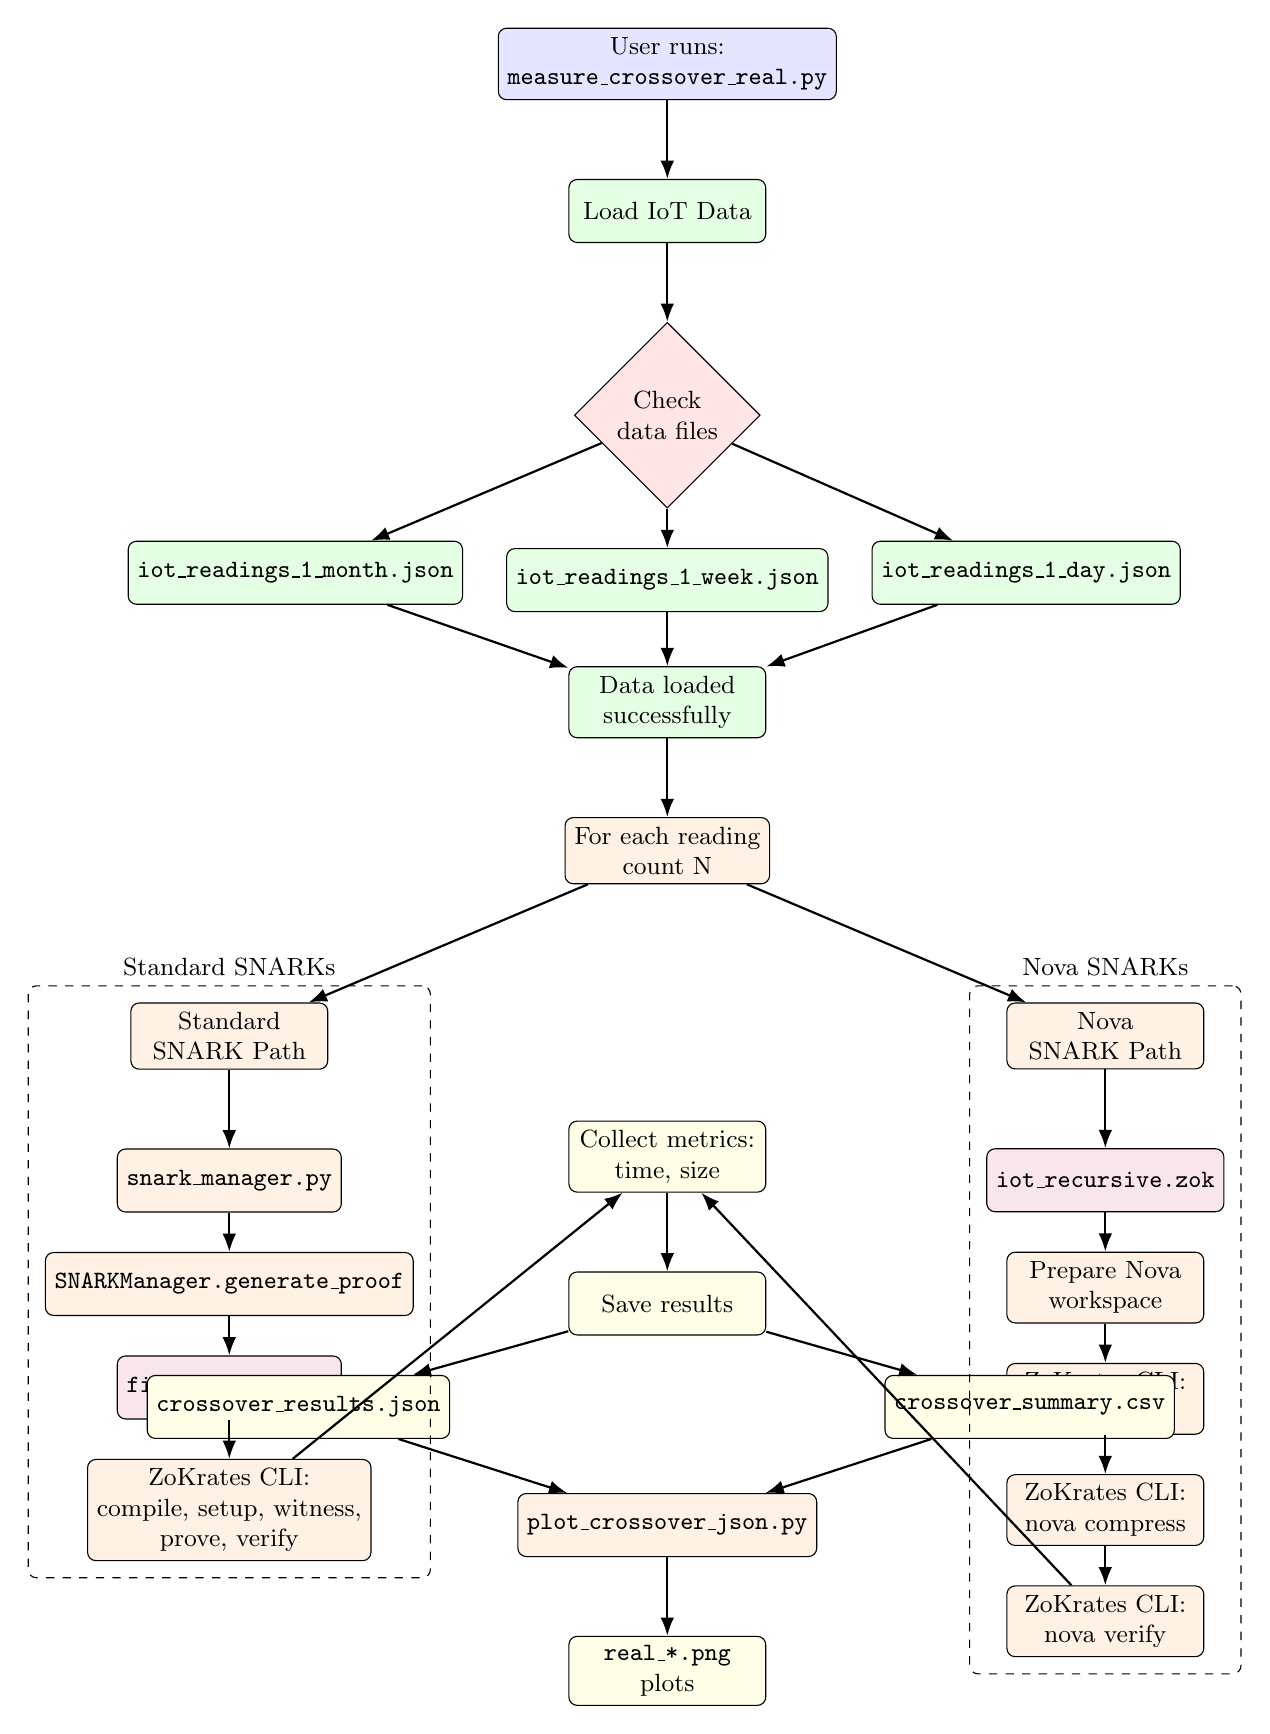
\begin{tikzpicture}[
  font=\small,
  start/.style={draw, rounded corners=3pt, align=center, minimum width=2.5cm, minimum height=0.8cm, fill=blue!10},
  data/.style={draw, rounded corners=3pt, align=center, minimum width=2.5cm, minimum height=0.8cm, fill=green!10},
  code/.style={draw, rounded corners=3pt, align=center, minimum width=2.5cm, minimum height=0.8cm, fill=orange!10},
  circuit/.style={draw, rounded corners=3pt, align=center, minimum width=2.5cm, minimum height=0.8cm, fill=purple!10},
  output/.style={draw, rounded corners=3pt, align=center, minimum width=2.5cm, minimum height=0.8cm, fill=yellow!10},
  decision/.style={diamond, draw, align=center, minimum width=1.5cm, minimum height=0.8cm, fill=red!10},
  arrow/.style={-Latex, thick},
  group/.style={draw, dashed, rounded corners=3pt, inner sep=6pt}
]

% Start
\node[start] (start) at (0,0) {User runs:\\\texttt{measure\_crossover\_real.py}};

% Data loading
\node[data, below=1cm of start] (load) {Load IoT Data};
\node[decision, below=1cm of load] (check) {Check\\data files};

% Data files
\node[data, below left=1cm and 2cm of check] (month) {\texttt{iot\_readings\_1\_month.json}};
\node[data, below=0.5cm of check] (week) {\texttt{iot\_readings\_1\_week.json}};
\node[data, below right=1cm and 2cm of check] (day) {\texttt{iot\_readings\_1\_day.json}};

% Data loaded
\node[data, below=2cm of check] (loaded) {Data loaded\\successfully};

% Loop
\node[code, below=1cm of loaded] (loop) {For each reading\\count N};

% Two paths
\node[code, below left=1.5cm and 3cm of loop] (std_path) {Standard\\SNARK Path};
\node[code, below right=1.5cm and 3cm of loop] (nova_path) {Nova\\SNARK Path};

% Standard SNARK components
\node[code, below=1cm of std_path] (snark_mgr) {\texttt{snark\_manager.py}};
\node[code, below=0.5cm of snark_mgr] (generate) {\texttt{SNARKManager.generate\_proof}};
\node[circuit, below=0.5cm of generate] (filter_circuit) {\texttt{filter\_range.zok}};
\node[code, below=0.5cm of filter_circuit] (zok_cli) {ZoKrates CLI:\\compile, setup, witness,\\prove, verify};

% Nova SNARK components
\node[circuit, below=1cm of nova_path] (nova_circuit) {\texttt{iot\_recursive.zok}};
\node[code, below=0.5cm of nova_circuit] (nova_workspace) {Prepare Nova\\workspace};
\node[code, below=0.5cm of nova_workspace] (nova_prove) {ZoKrates CLI:\\nova prove};
\node[code, below=0.5cm of nova_prove] (nova_compress) {ZoKrates CLI:\\nova compress};
\node[code, below=0.5cm of nova_compress] (nova_verify) {ZoKrates CLI:\\nova verify};

% Metrics collection
\node[output, below=3cm of loop] (metrics) {Collect metrics:\\time, size};

% Results
\node[output, below=1cm of metrics] (save) {Save results};
\node[output, below left=0.5cm and 1.5cm of save] (json) {\texttt{crossover\_results.json}};
\node[output, below right=0.5cm and 1.5cm of save] (csv) {\texttt{crossover\_summary.csv}};

% Visualization
\node[code, below=2cm of save] (plot) {\texttt{plot\_crossover\_json.py}};
\node[output, below=1cm of plot] (plots) {\texttt{real\_*.png}\\plots};

% Arrows
\draw[arrow] (start) -- (load);
\draw[arrow] (load) -- (check);
\draw[arrow] (check) -- (month);
\draw[arrow] (check) -- (week);
\draw[arrow] (check) -- (day);
\draw[arrow] (month) -- (loaded);
\draw[arrow] (week) -- (loaded);
\draw[arrow] (day) -- (loaded);
\draw[arrow] (loaded) -- (loop);
\draw[arrow] (loop) -- (std_path);
\draw[arrow] (loop) -- (nova_path);

% Standard path arrows
\draw[arrow] (std_path) -- (snark_mgr);
\draw[arrow] (snark_mgr) -- (generate);
\draw[arrow] (generate) -- (filter_circuit);
\draw[arrow] (filter_circuit) -- (zok_cli);

% Nova path arrows
\draw[arrow] (nova_path) -- (nova_circuit);
\draw[arrow] (nova_circuit) -- (nova_workspace);
\draw[arrow] (nova_workspace) -- (nova_prove);
\draw[arrow] (nova_prove) -- (nova_compress);
\draw[arrow] (nova_compress) -- (nova_verify);

% Metrics collection arrows
\draw[arrow] (zok_cli) -- (metrics);
\draw[arrow] (nova_verify) -- (metrics);
\draw[arrow] (metrics) -- (save);
\draw[arrow] (save) -- (json);
\draw[arrow] (save) -- (csv);
\draw[arrow] (json) -- (plot);
\draw[arrow] (csv) -- (plot);
\draw[arrow] (plot) -- (plots);

% Group boxes
\node[group, fit=(std_path)(snark_mgr)(generate)(filter_circuit)(zok_cli), label=above:{Standard SNARKs}] (std_group) {};
\node[group, fit=(nova_path)(nova_circuit)(nova_workspace)(nova_prove)(nova_compress)(nova_verify), label=above:{Nova SNARKs}] (nova_group) {};

\end{tikzpicture}
\end{document}
